%% ----------------------------------------------------------------
%% Thesis.tex -- MAIN FILE (the one that you compile with LaTeX)
%% ---------------------------------------------------------------- 

% Set up the document
\documentclass[a4paper, 11pt, oneside]{uet_thesis}  % Use the "Thesis" style, based on the ECS Thesis style by Steve Gunn
\graphicspath{{Figures/}}  % Location of the graphics files (set up for graphics to be in PDF format)

% Include any extra LaTeX packages required
\usepackage[square, numbers, comma, sort&compress]{natbib}  % Use the "Natbib" style for the references in the Bibliography

\usepackage{verbatim}  % Needed for the "comment" environment to make LaTeX comments
% \usepackage{vector}  % Allows "\bvec{}" and "\buvec{}" for "blackboard" style bold vectors in maths
\usepackage{url}
\usepackage{natbib}


\hypersetup{urlcolor=blue, colorlinks=true}  % Colours hyperlinks in blue, but this can be distracting if there are many links.

% remove the unnecessary spacing before and after the headings/subheadings
\usepackage[compact]{titlesec}
\titlespacing{\section}{0pt}{*0}{*0}
\titlespacing{\subsection}{0pt}{*0}{*0}
\titlespacing{\subsubsection}{0pt}{*0}{*0}

\setlength{\parskip}{6pt}
%\setlength{\parsep}{0pt}
%\setlength{\headsep}{0pt}
%\setlength{\topskip}{0pt}

%% ----------------------------------------------------------------
\begin{document}
\frontmatter	  % Begin Roman style (i, ii, iii, iv...) page numbering

% Set up the Title Page
\title  {Synopsis: Placement and Routing of UETRV-PCore}
%\session {2006 -- 2010}
\advisor {
	Prof. Suleman Sami Qasi % Add the name of co-supervisor under the name of supervisor by using \\ to go to new line.
}
\authors {
	2021-FYP-21\\
    \begin{tabular}{l l}
        Abdullah Azhar & 2021-EE-61\\
        Wajid Ali      & 2021-EE-79\\
        Uneeb Kamal    & 2021-EE-81\\
        Saad Gilani    & 2021-EE-118
    \end{tabular}
}

\addresses  {\deptname \\ \univname}  % Do not change this here, instead these must be set in the "Thesis.cls" file, please look through it instead
\date       {\today}
\subject    {}
\keywords   {}

\maketitle
%% ----------------------------------------------------------------

\setstretch{1.3}  % It is better to have smaller font and larger line spacing than the other way round

% Define the page headers using the FancyHdr package and set up for one-sided printing
\fancyhead{}  % Clears all page headers and footers
\rhead{\thepage}  % Sets the right side header to show the page number
\lhead{}  % Clears the left side page header

\pagestyle{fancy}  % Finally, use the "fancy" page style to implement the FancyHdr headers


\clearpage  % Certification ended, now start a new page

\setstretch{1.3}  % Reset the line-spacing to 1.3 for body text (if it has changed)


%% ----------------------------------------------------------------
\pagestyle{fancy}  %The page style headers have been "empty" all this time, now use the "fancy" headers as defined before to bring them back

%% ----------------------------------------------------------------
\lhead{\emph{Contents}}  % Sets the left side page header to "Contents"
\tableofcontents  % Write out the Table of Contents

%% ----------------------------------------------------------------
% \lhead{\emph{List of Figures}}  % Sets the left side page header to "List of Figures"
% \listoffigures  % Write out the List of Figures

%% ----------------------------------------------------------------
% \lhead{\emph{List of Tables}}  % Sets the left side page header to "List of Tables"
% \listoftables  % Write out the List of Tables

%% ----------------------------------------------------------------
\setstretch{1.5}  % Sets the line spacing to 1.5, this makes the following tables easier to read

\clearpage  % Start a new page

% \lhead{\emph{Abbreviations}}  % Sets the left side page header to "Abbreviations"
% \listofsymbols{ll}  % Includes a list of Abbreviations (a table of two columns)
% {
% % \textbf{Acronym} & \textbf{W}hat (it) \textbf{S}tands \textbf{F}or \\
% \textbf{LAH} & \textbf{L}ist \textbf{A}bbreviations \textbf{H}ere \\
% }

%% ----------------------------------------------------------------
% The Abstract Page
\addtotoc{Abstract}  % Adds the "Abstract" page entry to the Contents
\abstract{
%\addtocontents{toc}{\vspace{1em}}  % Adds a gap in the Contents, for aesthetics

This project focuses on the placement and routing of the UETRV-Pcore, a RISC-V-based system-on-chip (SoC). RISC-V is an open-source instruction set architecture (ISA). The core implements a pipelined architecture with essential stages such as instruction fetch, decode, execution, memory access, and writeback. The flow of the UETRV-Pcore follows the complete ASIC flow, starting from Register Transfer Level (RTL) design to the generation of a GDSII layout file for fabrication. Cadence Genus is used for logic synthesis, converting the RTL code into a gate-level netlist optimized for timing, area, and power. Cadence Innovus is employed for physical design, including key steps such as floorplanning, standard cell placement, power planning, clock tree synthesis, and routing. We use a 45nm generic process design kit (PDK) for implementing the design. This project highlights the challenges of modern VLSI design, including timing closure, power management, and layout optimization. It provides hands-on experience with industry-standard tools, offering valuable insights into the complexities of digital design flows. The final deliverable of this project is a fully verified GDSII file, which will be fabricated to produce the UETRV-Pcore chip. This project not only contributes to open-source hardware development but also serves as a foundation for future research in processor design and SoC development.

}
\clearpage  % Abstract ended, start a new page

%% ----------------------------------------------------------------
\mainmatter	  % Begin normal, numeric (1,2,3...) page numbering
\pagestyle{fancy}  % Return the page headers back to the "fancy" style
\onehalfspacing
% Include the chapters of the thesis, as separate files
% Just uncomment the lines as you write the chapters

% Chapter 1

\chapter{Introduction}
\label{Chapter1}

The UETRV-Pcore project is a groundbreaking initiative for Pakistan's academic and industrial sectors. So far, no student team has completed the entire RTL-to-GDS flow using Cadence tools for a complete SoC, which are widely used in the chip design industry. Our project, led by the Department of Electrical Engineering at UET Lahore, aims to fill this gap by developing a complete RISC-V-based application-class System-on-Chip (SoC). This effort is a first of its kind, as we are the pioneers in creating a GDSII (Graphic Data System) layout, the final stage of chip design required for fabrication.
Although Pakistan has a strong foundation in digital design and microarchitecture, the field of physical design and chip fabrication remains largely unexplored. By working on the UETRV-Pcore, we hope to set a new benchmark and encourage engineering programs across the country to focus on physical design. This project will also create opportunities for local chip design innovation and help improve Pakistan’s standing in the global semiconductor industry. If we successfully fabricate the UETRV-Pcore, it will not only validate our team’s expertise but also inspire students, researchers, and industries to explore chip design and fabrication leading to a major shift in the country’s technological landscape.
The UETRV-Pcore is a RISC-V-based application-class System-on-Chip (SoC). It integrates a 32-bit RISC-V ISA core, supporting RV32IMAZicsr instructions, which include base integer operations (I), multiplication and division (M), atomic operations (A), and control/status registers (Zicsr). The core implements three privilege levels—User (U), Supervisor (S), and Machine (M). With instruction and data caches and an SV32-based MMU (Memory Management Unit), UETRV-Pcore is capable of running Linux. The design features peripherals like UART, SPI, CLINT and PLIC that are connected via shared data buses. The design flow for UETRV-Pcore follows a structured physical design methodology using Cadence tools like Genus and Innovus. 
The first step in the physical design flow is synthesis, where the high-level Register Transfer Level (RTL) code is converted into a gate-level netlist. This is done using Cadence Genus, which performs technology mapping by replacing RTL constructs with logic gates from the 45nm standard cell library. Once synthesis is complete, the next step is floorplanning. In this stage, the major blocks of the design such as the core processor, caches, MMU, and peripherals are  placed logically within the chip area. It ensures that sufficient space is allocated for the components while minimizing wire lengths for efficient routing. In the placement stage, the standard cells from the synthesized netlist are placed onto the physical layout according to the floorplan. The tool ensures that the layout has no overlaps and creates space for clock distribution and routing tracks. This stage plays a critical role in improving the timing closure of the design. 
Clock Tree Synthesis (CTS) is one of the most critical stages of the physical design process. The objective of CTS is to create a balanced clock tree that distributes the clock signal uniformly across the chip with minimal clock skew and latency. Clock skew refers to the difference in the arrival time of the clock signal at various points in the design, which can cause timing violations if not controlled. Cadence Innovus uses buffer insertion and gating techniques to build an optimized clock tree. The tool ensures that the clock reaches all registers simultaneously, enabling synchronized operations across the pipeline stages. In the routing stage, the design tool connects the placed cells and peripherals through metal layers to form a complete circuit. During this process, the tool ensures that the design meets electrical rules, timing constraints, and power requirements. Design Rule Checking (DRC) and Layout vs. Schematic (LVS) verification are performed to confirm that the routed design matches the original schematic and complies with the manufacturing rules of the 45nm process.
 % Introduction 

% Chapter 2

\chapter{Problem Statement}
\label{Chapter2}
Unmet need or problem, what is the unmet need or problem the FYDP is aiming to solve? How significant is the problem? Quantify as much as possible. In case of a research problem, show the significance of the unsolved problem. Who needs it? List the type of customers who will be interested in the solution of the problem. For each type of customer, indicate the potential market size. In case of a research problem, identify its scope. ($1$ page) % Problem Statement

% Chapter 3

\chapter{Literature Review}
\label{Chapter3}

Huang et al. (2024) present a novel RTL-to-GDS automation flow specifically designed for adiabatic quantum-flux-parametron (AQFP) superconducting circuits. The authors detail how their custom approach optimizes design tasks at each stage of the flow, including synthesis, placement, and routing, tailored to the unique electrical characteristics of AQFP technologies \cite{huang2024superflow}. Although the focus is on a different circuit type, the core principles of customizing the design flow can be adapted to the UETRV-Pcore project. By analyzing the automation techniques described, the project can enhance its current flow using Cadence Genus and Innovus, potentially leading to better energy efficiency and performance in the RISC-V architecture. This paper serves as a critical reference for exploring custom automation in design flows, encouraging the adaptation of similar strategies for specific project needs.

Acharya and Mehta (2022) conducted a performance analysis comparing the open-source tool Qflow with the commercial tool Cadence Encounter for the RTL to GDS-II flow of a Synchronous FIFO design. They highlighted the accessibility of Qflow for students and researchers, allowing them to engage in projects without the financial burden of expensive commercial tools. Conversely, Cadence Encounter is noted for its efficiency and accuracy, making it a preferred choice in industrial applications. The study revealed that the number of standard cells required when using Qflow was 1.5 times greater than that of Cadence Encounter, resulting in an area requirement over 2.6 times larger. These findings underscore the trade-offs involved in selecting design tools, especially concerning area, power, and operating frequency. This work serves as a critical reference for understanding the implications of tool selection in the RTL to GDS-II process, providing valuable insights that will inform the design decisions for the UET-RV Pcore. \cite{acharya2022performance}

Dwight Hill and Andrew B. Kahng explore the complex journey of chip implementation from RTL (Register Transfer Level) description to GDSII (Graphic Data System II) data, essential for the tape-out process in chip design. They argue that chip implementation encompasses several critical stages, notably logic synthesis, placement, and routing (SP\&R), which have long been supported by advanced commercial tools. These tools have evolved significantly over the years, enabling design teams to refine their approaches through a spiraling methodology that enhances timing estimation, device placement, and accuracy in parasitic extraction. The authors highlight that much of the RTL-to-GDSII work is rooted in industrial practice rather than academic research. This trend is attributed to the complexity of the design process, which requires competitive technology across various software platforms—capabilities that are often beyond the scope of typical graduate projects. They note that the chip design flow involves multiple representations and thus is often referred to as physical synthesis. The process necessitates various libraries, including timing libraries that describe cell delay properties and physical libraries that define the geometry of logic cells and I/O buffers. Additionally, the authors emphasize that the complexity of timing constraints plays a vital role in the design implementation process, reflecting the critical need for timing closure. They discuss the inadequacies of traditional static timing analysis, which is typically conducted at the RTL handoff and mask sign-off milestones. In modern design flows, embedded timing analysis has become integral, driving the need for accurate timing abstractions throughout the entire implementation process \cite{hill2004guest}.

Hill and Kahng address the challenges posed by the non convergence of traditional flows, particularly as designs grow larger and more intricate. They identify various factors, such as crosstalk, substrate coupling, and thermal effects, that influence circuit timing and signal integrity. This complexity necessitates deeper integration between synthesis, analysis, and specification, which the authors argue is crucial for achieving predictable outcomes in chip design. The article presents three main categories of prediction methods aimed at improving design predictability. The first is statistical prediction, which, while quick, often lacks the required accuracy due to its reliance on average metrics. The second is constructive and iterative prediction, which involves real-time estimates based on previous design iterations. Lastly, the authors discuss the importance of enforced assumptions in design properties, which facilitate consistent outcomes throughout the design process \cite{hill2004guest}.
 % Literature Review

% Chapter 4

\chapter{Project Overview and Objectives}
\label{Chapter4}

The primary objective of this project is to complete the design and physical implementation of the UETRV-Pcore, a RISC-V-based System-on-Chip (SoC), using a structured ASIC flow. The specific objectives are:
\begin{itemize}
    \item End-to-End ASIC Flow Implementation: To implement the UETRV-Pcore from Register Transfer Level (RTL) to a GDSII layout file, covering all key stages of physical design.
    \item Optimization for Timing, Area, and Power: To synthesize the RTL code into a gate-level netlist optimized for timing, area, and power using Cadence Genus.
    \item Physical Layout and Routing: To perform physical design steps including floorplanning, placement, clock tree synthesis, and routing using Cadence Innovus.
    \item Fabrication-Ready GDSII: To generate a verified GDSII layout file that meets design rule checks (DRC) and layout vs. schematic (LVS) checks, making the design ready for fabrication.
    \item Contribute to Open-Source Hardware: To contribute to the global RISC-V and open-source hardware community by creating a fabricatable, open-source processor design.
\end{itemize}




 % Project Overview and Objectives

% Chapter 5

\chapter{Project Development Methodology/Architecture}
\label{Chapter5}

The proposed solution for achieving the objectives is to implement the UETRV-Pcore by following a detailed ASIC design flow using industry-standard tools:
\begin{itemize}
    \item RTL Design: A RISC-V 32-bit processor core implementing the RV32IMAZicsr instruction set architecture (ISA) will be designed. It will include a pipelined architecture with essential stages like instruction fetch, decode, execution, memory access, and writeback.
    \item Synthesis: The RTL design will be synthesized using Cadence Genus, which will optimize the design for area, timing, and power using the 45nm standard cell library.
    \item Floorplanning and Placement: The major blocks, such as the processor core, caches, MMU, and peripherals (UART, SPI, CLINT, and PLIC), will be floorplanned and placed logically within the chip area. The placement of standard cells will be optimized to minimize wire lengths and improve timing.
    \item Clock Tree Synthesis and Routing: A balanced clock tree will be created using Cadence Innovus to ensure uniform clock distribution with minimal skew and latency. The tool will then route the design to connect the cells and peripherals, ensuring it meets electrical, timing, and power requirements.
    \item Verification and Sign-Off: The routed design will undergo Design Rule Checking (DRC) and Layout vs. Schematic (LVS) verification to ensure compliance with manufacturing rules and match the original schematic.
    \item GDSII Generation: The final verified design will be exported as a GDSII layout file, ready for fabrication.

\end{itemize} % Project Development Methodology/Architecture

% Chapter 6

\chapter{Project Milestones and Deliverables}
\label{Chapter6}

\begin{enumerate}
    \item Synthesis
    \item Floor-planning
    \item Placement
    \item Routing
    \item Complete GDS
\end{enumerate} % Project Milestones and Deliverables

% Chapter 7

\chapter{Block Diagram}
\label{Chapter7}

Draw a block diagram of your project and explain it briefly. ($1$ page) % Block Diagram

% Chapter 8

\chapter{Flow Chart}
\label{Chapter8}

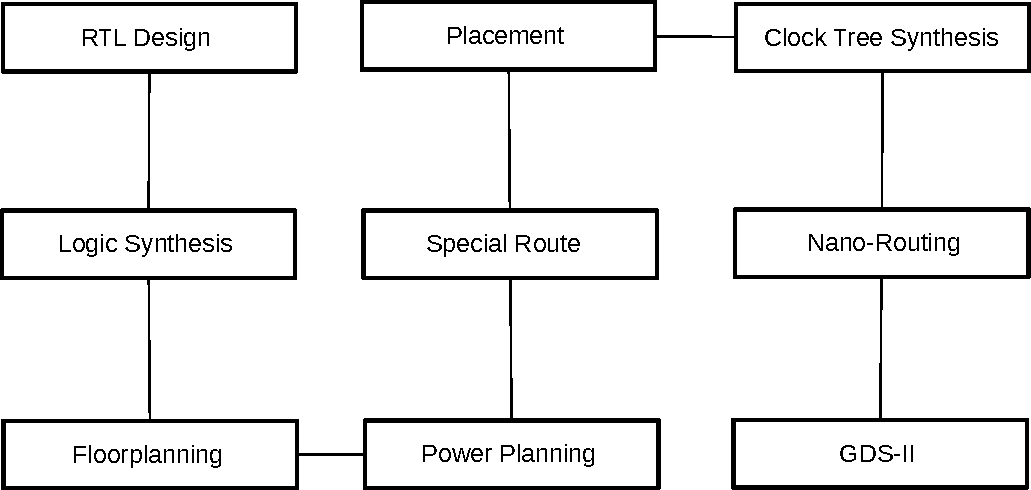
\includegraphics[width=\textwidth]{flow_chart.pdf} % Flow Chart

% Chapter 9

\chapter{Work Division}
\label{Chapter9}

Clear work division among group members must be indicated. ($1$ page) % Work Division

% Chapter 10

\chapter{Costing}
\label{Chapter10}

Cadence VLSI \$6,500 USD annually, Sponsored by NCDC of NUST. % Costing

%% ----------------------------------------------------------------

%% ----------------------------------------------------------------
\addtocontents{toc}{\vspace{2em}}  % Add a gap in the Contents, for aesthetics
\backmatter

\bibliographystyle{plainnat}  % Use "unsrtnat" BibTeX style for formatting the references

\bibliography{references}  % The references information is stored in the file named "references.bib"

\end{document}  % The End
%% ----------------------------------------------------------------
